\section{Study Design}

This experiment will focus on training the user to improve prosthetic control on a fixed pattern recognition-based control system. The novel approach in this study is to provide the user with information on how well the system recognizes the performed movement during user training by showing the uncertainty of recognized movement as a visual feedback. The following section will lay an overview of the implementation of the different stages of this experiment.

To test if myoelectric prosthetic control can be improved by using a visual uncertainty feedback the following research hypothesis has been made.  
\begin{center}
	Exposing subjects to user training, in which confidence levels of movement recognition is used as feedback, will show improvement in performance in a classification-based myoelectric prosthetic control scheme compared the control group.
\end{center}

To test the hypothesis XX subjects of age XX $\pm$ XX were recruited, X right handed and X left handed, and randomly assigned to either a control group or test group. The subjects enrolled were assessed to meet inclusion criteria presented in the experimental protocol for test subjects in \secref{sec:Eprot}. The experimental protocol was handed out to possible test participants before enrollment. The experiment is designed as a three session trail where data is acquired for both control and test group, receiving user training and gets a performance a test taken in all sessions. It is important that during the experiment the subject will be placed sitting on a chair, with the arm, wearing the MYB on their dominant arm, hanging relaxed down by the side of the body. A graphical illustration of the stages of the experiment design can be seen on \figref{fig:std}. Essential for the experiment is the difference in user training highlighted in step 3 where the groups will receive two different kinds of visual feedback. The sections to come will further chronologically elaborate on the implementation of each element in the experiment.          
 

\begin{figure}[H]                                         
	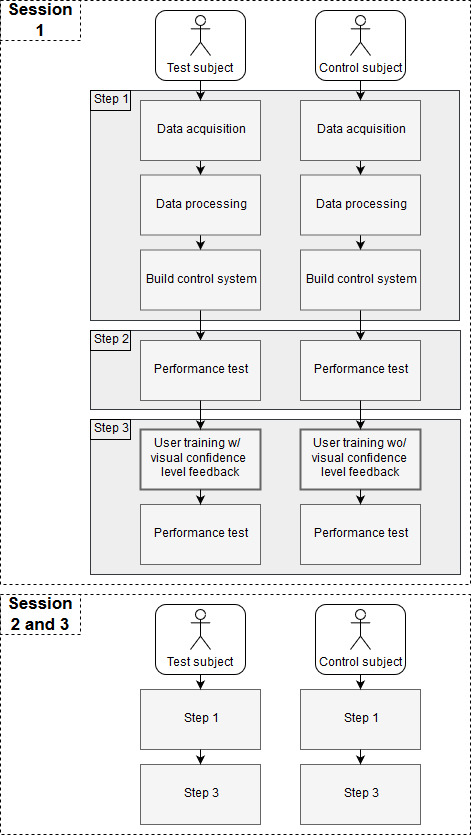
\includegraphics[width=.64\textwidth]{figures/pMethods/Study_design}  
	\caption{Graphical illustration of the experiment showing the steps of each session for the test and control group. Highlighted is user training in step three which essentially is the only place where the experiment differs between groups in the type of feedback given.}
	\label{fig:std} 
\end{figure}   


